\documentclass[10pt, aspectratio=169]{beamer}

\usetheme[progressbar=frametitle, sectionpage=progressbar, subsectionpage=progressbar, numbering=fraction, block=fill]{metropolis}

\definecolor{mLightBrown}{HTML}{4D4D4D}
\definecolor{mMediumBrown}{HTML}{2C2C2A}
\definecolor{mDarkBrown}{HTML}{1A1A19}
\definecolor{mDarkTeal}{HTML}{0F6E56}
\definecolor{mDarkRed}{HTML}{B03A2E}
\setbeamercolor{normal text}{fg=mDarkBrown}
\setbeamercolor{alerted text}{fg=mDarkTeal}
\setbeamercolor{frametitle}{bg=mDarkBrown}
\setbeamercolor{progress bar}{fg=mDarkTeal, bg=mDarkTeal!20}
\definecolor{mPaleBg}{HTML}{F4F3EE}
\setbeamercolor{block title}{bg=mDarkBrown!10, fg=mDarkBrown}
\setbeamercolor{block body}{bg=mPaleBg, fg=mDarkBrown}
\newcommand{\hl}[1]{\textcolor{mDarkTeal}{#1}}

\usepackage{amsmath, amssymb, amsthm, mathtools}
\usepackage{cancel}\usepackage{bm}\usepackage{booktabs}\usepackage{array}
\usepackage{xcolor}\usepackage{colortbl}\usepackage{multirow}\usepackage{tikz}
\usetikzlibrary{positioning,arrows.meta,calc,fit,shapes.geometric,decorations.pathmorphing}

\newcommand{\paper}[1]{\textcolor{mLightBrown}{\small\textit{(#1)}}}

\newcommand{\qcur}{0}
\newcommand{\qnode}[4]{%
\ifnum#4=\qcur
 \node[draw=mDarkTeal, fill=mDarkTeal!12, thick, rounded corners=1pt, minimum width=3.0cm, minimum height=0.52cm, font=\tiny\bfseries, text=mDarkBrown] (#2) at (#1,0) {#3};%
\else
 \node[draw=mLightBrown!45, rounded corners=1pt, minimum width=3.0cm, minimum height=0.52cm, font=\tiny, text=mLightBrown] (#2) at (#1,0) {#3};%
\fi}
\newcommand{\qstrip}[1]{\renewcommand{\qcur}{#1}%
\begin{center}
\begin{tikzpicture}
\qnode{0}{q1}{Q1 Invert?}{1}
\qnode{3.7}{q2}{Q2 Generate?}{2}
\qnode{7.4}{q3}{Q3 VAE?}{3}
\qnode{11.1}{q4}{Q4 Condition?}{4}
\draw[-{Stealth}, mLightBrown!60] (q1.east) -- (q2.west);
\draw[-{Stealth}, mLightBrown!60] (q2.east) -- (q3.west);
\draw[-{Stealth}, mLightBrown!60] (q3.east) -- (q4.west);
\end{tikzpicture}\end{center}}

\title{Data-Driven Design Optimization --- Generative-Based}
\subtitle{Don't search the design --- produce it}
\author{Jinkyoo Park}
\institute{KAIST}
\date{\textit{Lecture 6 --- Offline optimization, part 2 of 2: invert the function, then sample}}

\begin{document}

\maketitle

%==========================================================
\section{The handoff --- the same problem, inverted}
%==========================================================

\begin{frame}{Where we are --- the dual of last lecture}
\vspace{2pt}
The problem is unchanged from Lecture 5 --- word for word:
\[
\text{find}\quad x^* = \arg\max_x f(x) \qquad \text{with \alert{only} a fixed dataset } D = \{(x_i, f(x_i))\}_{i=1}^N.
\]
\medskip

\pause
Lecture 5 took the \alert{forward} route: approximate $f_\theta(x)\approx f(x)$, then \emph{search} it for a maximum (guarding against the surrogate's blind spots). This lecture takes the opposite route:
\medskip
\begin{center}\large
learn the \alert{inverse} map --- from a desired output to an input that achieves it --- and \alert{sample} from it.
\end{center}
\medskip

\pause
\begin{center}\footnotesize\renewcommand{\arraystretch}{1.45}
\begin{tabular}{l|c|c}
 & \textbf{model} & \textbf{decision} \\
\hline
\textbf{Surrogate (Lec.\ 5)} & forward $f_\theta(x)$ & \alert{search} for the max \\
\textbf{Generative (Lec.\ 6)} & \cellcolor{mDarkTeal!15}inverse $p(x\mid y)$ & \cellcolor{mDarkTeal!15}\alert{sample} a good design \\
\end{tabular}
\end{center}
\end{frame}

\begin{frame}{The thesis --- generate, don't search}
The fixed point of this lecture, in one line:
\begin{center}\large
\alert{Instead of asking ``which input scores highest?'', model ``what do high-scoring inputs look like?'' --- and draw one.}
\end{center}
\medskip

\pause
Formally, jointly model $p(x,y) = p(y\mid x)\,p(x)$ and then sample from the conditional
\[
x \sim p\big(x \mid y \ge y_{\max}\big) \qquad (\text{more generally } p(x\mid S) \text{ for a target set } S).
\]
\medskip

\pause
Two ingredients make this work, and they are the lecture:
\begin{itemize}\setlength\itemsep{1pt}
\item a \alert{generative model} of valid designs --- the prior $p(x)$, learned so samples stay on the narrow valid manifold;
\item an \alert{inversion} mechanism --- conditioning that prior on ``good outcome.''
\end{itemize}
\pause
The narrow-manifold problem that doomed naive search (Lecture 5) is here handled \emph{by construction}: a generative model only ever produces on-manifold designs.
\end{frame}

\begin{frame}{The roadmap --- four questions}
\qstrip{0}
\medskip
\begin{itemize}\setlength\itemsep{3pt}
\item \textbf{Q1 --- What does inverting the function mean?} Learn $p(x\mid y)$, train it by divergence matching.
\item \textbf{Q2 --- How do we model valid designs at all?} \alert{Generative models} --- a prior $p(x)$.
\item \textbf{Q3 --- One concrete model.} The \alert{VAE}: encoder, decoder, latent $z$.
\item \textbf{Q4 --- How do we steer toward \emph{good} designs?} \alert{Conditioning} --- Model Inversion Networks.
\end{itemize}
\end{frame}

%==========================================================
\section{Act 1 --- inverting the function}
%==========================================================

\begin{frame}{The inverse map --- from outcome back to design}
\qstrip{1}
\medskip
The forward model answers ``given $x$, what is $y$?''. The \alert{inverse} model answers the question we actually care about: ``given a desired $y$, what $x$ produces it?''
\medskip

Train an inverse map $f^{-1}_\theta(x\mid y)$ to match the data's conditional, by minimizing a divergence:
\[
L_p(D) = \mathbb{E}_{y\sim p(y)}\Big[\,\mathrm{Div}\big(\,p_D(x\mid y)\;,\; p_{f^{-1}_\theta}(x\mid y)\,\big)\Big].
\]
\medskip

\pause
The choice of divergence recovers familiar training objectives:
\begin{itemize}\setlength\itemsep{1pt}
\item \textbf{KL divergence} $\Rightarrow$ maximum-likelihood training of the inverse map;
\item \textbf{JS divergence} $\Rightarrow$ a GAN-style adversarial objective.
\end{itemize}
\medskip

\pause
\begin{center}\large
Searching is replaced by \alert{conditioning}: set $y$ high, read off $x$.
\end{center}
But $x$ lives in a high-dimensional space where only a thin manifold is valid --- so the inverse map must be backed by a model that \emph{knows what valid $x$ looks like}. Enter generative models.
\end{frame}

%==========================================================
\section{Act 2 --- generative models}
%==========================================================

\begin{frame}{Generative models --- learning the manifold of valid designs}
\qstrip{2}
\medskip
\begin{block}{The goal}
\centering
Train $p_\theta(x)$ to match the data distribution $p_{\text{data}}(x)$, given samples $\{x_i\}\sim p_{\text{data}}$.
\end{block}
\medskip

A generative model maps simple noise $z\sim\mathcal{N}(0,I)$ to realistic samples $x$ --- learning the \alert{narrow valid manifold} as the support of $p_\theta$.
\medskip

\pause
\begin{center}\footnotesize\renewcommand{\arraystretch}{1.4}
\begin{tabular}{l|l}
\textbf{Family} & \textbf{Mechanism} \\
\hline
Variational Autoencoder (VAE) & encode to latent, decode; maximize a variational bound \\
GAN & generator vs.\ discriminator (adversarial) \\
Normalizing flow & invertible transform of a simple density \\
Diffusion model & add Gaussian noise, then learn to reverse it \\
\end{tabular}
\end{center}
\medskip

\pause
Any of these can serve as the prior $p(x)$ over designs. We take the VAE as the worked example --- it makes the latent variable, and the inversion, most explicit.
\end{frame}

%==========================================================
\section{Act 3 --- the VAE}
%==========================================================

\begin{frame}{The Variational Autoencoder --- encode, decode, generate}
\qstrip{3}
\medskip
\begin{center}
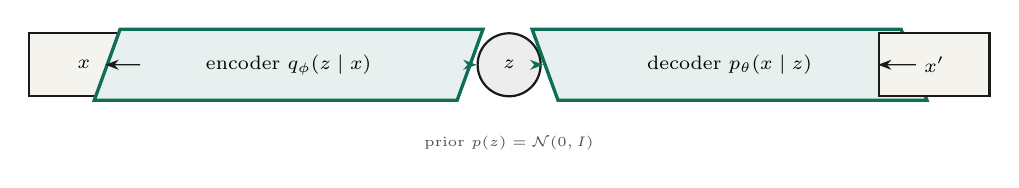
\begin{tikzpicture}[font=\scriptsize, node distance=8pt]
\node[draw=mDarkBrown, thick, fill=mPaleBg, minimum width=1.4cm, minimum height=0.8cm] (x) at (0,0) {$x$};
\node[draw=mDarkTeal, very thick, fill=mDarkTeal!10, trapezium, trapezium left angle=70, trapezium right angle=110, minimum height=0.9cm] (enc) at (2.6,0) {encoder $q_\phi(z\mid x)$};
\node[draw=mDarkBrown, thick, fill=mDarkBrown!8, circle, minimum size=0.8cm] (z) at (5.4,0) {$z$};
\node[draw=mDarkTeal, very thick, fill=mDarkTeal!10, trapezium, trapezium left angle=110, trapezium right angle=70, minimum height=0.9cm] (dec) at (8.2,0) {decoder $p_\theta(x\mid z)$};
\node[draw=mDarkBrown, thick, fill=mPaleBg, minimum width=1.4cm, minimum height=0.8cm] (xr) at (10.8,0) {$x'$};
\draw[-{Stealth}, mDarkBrown] (x)--(enc); \draw[-{Stealth}, mDarkTeal] (enc)--(z);
\draw[-{Stealth}, mDarkTeal] (z)--(dec); \draw[-{Stealth}, mDarkBrown] (dec)--(xr);
\node[mLightBrown, font=\tiny] at (5.4,-1.0) {prior $p(z)=\mathcal{N}(0,I)$};
\end{tikzpicture}
\end{center}
\medskip
\begin{itemize}\setlength\itemsep{1pt}
\item \textbf{Generative process:} sample $z\sim\mathcal{N}(0,I)$, decode $x = p_\theta(x\mid z)$ --- this is how we \emph{produce} new designs.
\item \textbf{Inference:} the encoder $q_\phi(z\mid x)$ approximates the intractable posterior $p(z\mid x)$.
\end{itemize}
\medskip

\pause
Train both by maximizing the \alert{evidence lower bound} (ELBO):
\[
\mathcal{L}_{\theta,\phi}(x) = \mathbb{E}_{q_\phi(z\mid x)}\big[\log p_\theta(x\mid z)\big] - \mathrm{KL}\big(q_\phi(z\mid x)\,\|\,p(z)\big).
\]
\end{frame}

\begin{frame}{Reading the ELBO --- reconstruct, and stay regular}
\[
\mathcal{L}_{\theta,\phi}(x) = \underbrace{\mathbb{E}_{q_\phi(z\mid x)}\big[\log p_\theta(x\mid z)\big]}_{\text{\hl{reconstruction}}} - \underbrace{\mathrm{KL}\big(q_\phi(z\mid x)\,\|\,p(z)\big)}_{\text{\hl{stay near the prior}}}.
\]
\medskip
\begin{itemize}\setlength\itemsep{2pt}
\item the \textbf{reconstruction} term: the decoded $x'$ should match the input $x$ --- the model must actually capture the data;
\item the \textbf{KL} term: the encoded latents should look like the prior $\mathcal{N}(0,I)$ --- so that sampling $z$ from the prior at generation time lands in a region the decoder understands.
\end{itemize}
\medskip

\pause
\begin{center}\large
The KL term is what makes the latent space \alert{samplable} --- a smooth, prior-shaped code from which new valid designs can be drawn.
\end{center}
\medskip
\pause
{\footnotesize\textcolor{mLightBrown}{This is Lecture 2's full-Bayes idea --- a latent prior, a likelihood, a variational posterior --- scaled to a deep model. Diffusion models are a VAE with a fixed, multi-step Gaussian encoder; the same lower-bound logic underlies them.}}
\end{frame}

%==========================================================
\section{Act 4 --- conditioning toward good designs}
%==========================================================

\begin{frame}{Model Inversion Networks --- sampling the \emph{good} designs}
\qstrip{4}
\medskip
A generative model gives us valid designs; we want valid \emph{and high-scoring} designs. \alert{Model Inversion Networks} (MINs) supply the inversion. \paper{Kumar \& Levine, 2019}
\medskip

\pause
\textbf{The pieces.}
\begin{itemize}\setlength\itemsep{1pt}
\item a \emph{forward} model / oracle $p(y\mid x)$ (possibly a black box) --- ``how good is this design?'';
\item a generative \emph{prior} $p(x)$ over valid designs (Act 2--3);
\item together they define the joint $p(x,y)=p(y\mid x)p(x)$, and hence the conditional $p(x\mid y)$.
\end{itemize}
\medskip

\pause
\textbf{The query.} Train an inverse map $x = f^{-1}_\theta(y, z)$ (with noise $z$ for diversity), then sample designs conditioned on a high target:
\[
x \sim p\big(x \mid y \ge y_{\max}\big).
\]
\medskip
\pause
\begin{center}\large
Set the bar high, sample below it --- and out come candidate designs, on-manifold by construction.
\end{center}
\end{frame}

\begin{frame}{Why generation sidesteps the surrogate trap}
Recall Lecture 5's failure: gradient ascent climbed into out-of-distribution hallucinations because nothing kept it on the valid manifold.
\medskip

\pause
The generative approach removes that failure mode \alert{structurally}:
\begin{itemize}\setlength\itemsep{2pt}
\item it never optimizes \emph{over} input space, so there is no ascent to run off-manifold;
\item every output is a \emph{sample} from a model of \emph{valid} designs --- on-manifold by definition;
\item conditioning on $y\ge y_{\max}$ steers toward good designs \emph{within} that valid set.
\end{itemize}
\medskip

\pause
\begin{block}{The trade}
\centering
Surrogate search risks invalid designs but optimizes sharply. \\
Generative sampling guarantees valid designs but is bounded by what the data's good region contains.
\end{block}
\medskip
\pause
Neither dominates --- they are two faces of one offline problem, and a practitioner often uses both: a generative prior to stay valid, a (conservative) surrogate to rank.
\end{frame}

%==========================================================
\section{Closing}
%==========================================================

\begin{frame}{Where we are --- the design-optimization duality, complete}
\vspace{2pt}
\begin{center}\footnotesize\renewcommand{\arraystretch}{1.45}
\begin{tabular}{l|c|c}
 & \textbf{Surrogate (Lec.\ 5)} & \textbf{Generative (Lec.\ 6)} \\
\hline
direction & forward $f_\theta(x)$ & inverse $p(x\mid y)$ \\
decision & \alert{search} for the max & \alert{sample} a design \\
valid manifold & guarded (conservatism) & enforced (by construction) \\
risk & off-manifold hallucination & limited to data's good region \\
\end{tabular}
\end{center}
\medskip

\pause
\begin{center}\large
\alert{Search vs.\ produce} --- the same problem, attacked from opposite ends.
\end{center}
\medskip

\pause
Remember this duality. It is about to return, one level up, as the deepest split in reinforcement learning: \alert{value-based RL searches a value} ($\arg\max_a Q$, like Lecture 5's search) while \alert{policy-based RL produces an action} ($\pi_\theta(a\mid s)$, like Lecture 6's generation).
\end{frame}

\begin{frame}{Closing --- the one sentence}
\vfill
\begin{center}\large
To optimize a function you only have as data,\\[6pt]
you can approximate it and \alert{search} (Lecture 5) ---\\[4pt]
or model its inverse and \alert{sample} (Lecture 6).\\[8pt]
Forward and search, or inverse and produce:\\[4pt]
the two ways to turn data into a decision.
\end{center}
\vfill
\pause
\footnotesize
With Lecture 6, Part III closes --- and so does the static half of the course. Every problem so far was a single decision. Lecture 7 lets the decision unfold over time, and the value function is born.
\end{frame}

\begin{frame}[standout]
Questions?
\end{frame}

%==========================================================
\appendix
%==========================================================

\begin{frame}{Backup 1 --- the VAE objective, derived}
\footnotesize
We want to maximize the log-evidence $\log p_\theta(x)$, but it is intractable (it integrates over $z$). Introduce a variational posterior $q_\phi(z\mid x)$ and apply Jensen / the KL identity:
\[
\log p_\theta(x) = \underbrace{\mathbb{E}_{q_\phi}\Big[\log\tfrac{p_\theta(x,z)}{q_\phi(z\mid x)}\Big]}_{\text{ELBO } \mathcal{L}_{\theta,\phi}(x)} + \underbrace{\mathrm{KL}\big(q_\phi(z\mid x)\,\|\,p_\theta(z\mid x)\big)}_{\ge 0}.
\]
Since the KL is non-negative, the ELBO is a \emph{lower bound} on $\log p_\theta(x)$; maximizing it both fits the data and drives $q_\phi$ toward the true posterior. Expanding $p_\theta(x,z)=p_\theta(x\mid z)p(z)$ gives the working form
\[
\mathcal{L}_{\theta,\phi}(x) = \mathbb{E}_{q_\phi(z\mid x)}[\log p_\theta(x\mid z)] - \mathrm{KL}(q_\phi(z\mid x)\,\|\,p(z)). \quad\blacksquare
\]
\textbf{Reparameterization.} To backprop through the sampling $z\sim q_\phi$, write $z = \mu_\phi(x) + \sigma_\phi(x)\odot\epsilon$, $\epsilon\sim\mathcal{N}(0,I)$ --- moving the randomness off the parameters so gradients flow.
\end{frame}

\begin{frame}{Backup 2 --- the generative-model families, compared}
\footnotesize
\begin{center}\scriptsize\renewcommand{\arraystretch}{1.4}
\begin{tabular}{l|l|l|l}
\textbf{Family} & \textbf{Training} & \textbf{Latent} & \textbf{Trade-off} \\
\hline
VAE & maximize ELBO & explicit, $\sim\mathcal{N}(0,I)$ & stable; samples can be blurry \\
GAN & adversarial (gen.\ vs.\ disc.) & implicit & sharp; unstable, mode collapse \\
Normalizing flow & exact max-likelihood & invertible, same dim & exact density; architectural constraints \\
Diffusion & denoising score matching & noise schedule (fixed) & high quality; slow sampling \\
\end{tabular}
\end{center}
\medskip
\textbf{Diffusion as a VAE.} A diffusion model is a hierarchical VAE whose ``encoder'' is a \emph{fixed} multi-step Gaussian noising process (no parameters to learn), whose latents share the data's dimension, and whose top-level prior is $\mathcal{N}(0,I)$. The reverse (denoising) process is the learned decoder, trained by the same evidence-lower-bound logic --- which is why all four families serve interchangeably as the prior $p(x)$ in a generative design pipeline.
\end{frame}

\begin{frame}{Backup 3 --- MINs: training and querying the inverse map}
\footnotesize
\textbf{Training.} Learn $f^{-1}_\theta(x\mid y)$ to match the data's conditional by minimizing a divergence,
\[
L_p(D) = \mathbb{E}_{y\sim p(y)}\big[\mathrm{Div}(p_D(x\mid y),\, p_{f^{-1}_\theta}(x\mid y))\big],
\]
with KL $\Rightarrow$ maximum likelihood, JS $\Rightarrow$ GAN-style adversarial training. A noise input $z$ gives the map stochasticity so that, for a single $y$, it can produce a \emph{diversity} of valid designs (the conditional is one-to-many).
\medskip
\textbf{Querying.} At test time, choose a target value above anything seen (or a target set $S$) and sample:
\[
x \sim p\big(x\mid y\ge y_{\max}\big), \qquad x = f^{-1}_\theta(z, y_{\text{target}}),\ z\sim\mathcal{N}(0,I).
\]
\textbf{The subtlety.} Querying \emph{above} the data range is extrapolation --- the same off-distribution hazard as Lecture 5, now in output space. Practical MINs temper $y_{\text{target}}$ and re-rank samples with a (conservative) forward model, marrying the two halves of Part III into one pipeline: generate to stay valid, score to select.
\end{frame}

\end{document}
